\section{Connectedness}
\label{sect:connectedness}
\subsection{Connectedness}
\begin{enumerate}
\item We have generalized the \emph{extreme value theorem} in
\Cref{thm:cts-cpt-evt}. Then the next natural thing to do is to generalize the
\emph{intermediate value theorem} we learn in MATH2241. It turns out that the
generalization uses the notion of \emph{connectedness}.

\item It is somehow complicated to directly define the concept of
connectedness. So, we shall first define the notion of
\underline{dis}connectedness, and then define connectedness as the state of
being \emph{not} disconnected.

\item A metric space \(X\) is said to be \defn{disconnected} if \(X=A\sqcup B\)
for some nonempty and disjoint sets \(A\) and \(B\) which are open in \(X\).  A
metric space \(X\) is said to be \defn{connected} if it is not disconnected. A
subset \(S\) of \(X\) is said to be \defn{connected} (in \(X\)) if it is
connected when considered as a metric space itself under the induced metric.

Example: \(X=[0,1]\cup [2,3]\) (equipped with standard Euclidean metric) is
disconnected, by noting that \([0,1]\) and \([2,3]\) are nonempty disjoint open
subsets of \(X\) whose union is \(X\).

\item The following gives several criteria for being disconnected.

\begin{proposition}
\label{prp:discon-crit}
Let \(X\) be a metric space. The following are equivalent.
\begin{enumerate}
\item \(X\) is disconnected, i.e., \(X=A\sqcup B\) for some nonempty and
disjoint sets \(A\) and \(B\) which are \emph{open} in \(X\).
\item \(X=A\sqcup B\) for some nonempty and
disjoint sets \(A\) and \(B\) which are \emph{closed} in \(X\).
\item There exists a proper nonempty closed and open subset of \(X\).
\end{enumerate}
\end{proposition}
\begin{pf}
\underline{\(\text{(a)}\implies \text{(b)}\)}: Assume that \(X=A\sqcup B\) for some nonempty and
disjoint sets \(A\) and \(B\) which are \emph{open} in \(X\). Note that as
complements of each other, \(B=X\setminus A\) and \(A=X\setminus B\) are also
\emph{closed} in \(X\).

\underline{\(\text{(b)}\implies \text{(c)}\)}: Assume that \(X=A\sqcup B\) for
some nonempty and disjoint sets \(A\) and \(B\) which are \emph{closed} in
\(X\). Then \(A=X\setminus B\) is open in \(X\). Since \(B\) is nonempty,
\(A=X\setminus B\) is a \emph{proper} subset of \(X\). It then follows that
\(A\) is a proper nonempty closed and open subset of \(X\).

\underline{\(\text{(c)}\implies \text{(a)}\)}: Assume that there exists a
proper nonempty closed and open subset of \(X\). Define \(B=X\setminus A\).
Since \(A\) is a \emph{proper} subset of \(X\), the set \(B\) is nonempty.
Furthermore, since \(A\) is closed in \(X\), \(B=X\setminus A\) is open in
\(X\). Also, we can see that \(A\cap B=\varnothing\) and \(X=A\sqcup B\).
\end{pf}

\item Proving that a metric space is \underline{dis}connected is usually not
too difficult, since all we need to do is to find an example of \(A\) and \(B\)
satisfying the specified conditions. On the other hand, it is much more
difficult to prove that a metric space is connected, since we need to show that
there \emph{do not exist} any such sets \(A\) and \(B\). We need to consider all
possible choices!

To simplify the arguments, the use of a continuous function which takes only
two possible values is very helpful.

\item Any continuous function from \(X\) to \(\{0,1\}\) equipped with discrete
metric is called a \defn{2-valued function} on \(X\). The following result
suggests how 2-valued function can help us to prove connectedness.

\begin{theorem}
\label{thm:conn-2-val}
A metric space \(X\) is connected iff the only possible 2-valued functions on
\(X\) are constant functions.
\end{theorem}
\begin{pf}
``\(\Leftarrow\)'': We prove by contrapositive. Assume that \(X\) is
disconnected. Then we can write \(X=A\sqcup B\) for some nonempty and disjoint
sets \(A\) and \(B\) which are open in \(X\). Then define a function
\(f:X\to\{0,1\}\), where \(\{0,1\}\) is equipped with discrete metric, by
\[
f(x)=\begin{cases}
0&\text{if \(x\in A\)},\\
1&\text{if \(x\in B\)}.
\end{cases}
\]
Note that every subset of \(\{0,1\}\) is open.  Then we can check that
\(f^{-1}(\varnothing)=\varnothing\), \(f^{-1}(\{0\})=A\), \(f^{-1}(\{1\})=B\), and
\(f^{-1}(\{0,1\})=A\sqcup B=X\) are all open in \(X\). Thus, \(f\) is
continuous, hence is a non-constant 2-valued function.


``\(\Rightarrow\)'': Assume that \(X\) is connected.  Let \(f:X\to\{0,1\}\) be
a 2-valued function. Assume to the contrary that \(f\) is non-constant. Then
the preimages \(f^{-1}(\{0\})\) and \(f^{-1}(\{1\})\) are both nonempty. Also,
due to the continuity of \(f\), the preimages are both open in \(X\). Note also
that \(f^{-1}(\{0\})\cap f^{-1}(\{1\})=\varnothing\). Thus, we can write
\[
X=f^{-1}(\{0\})\sqcup f^{-1}(\{1\}),
\]
which implies that \(X\) is disconnected, contradiction.
\end{pf}

\item Like compactness, \emph{connectedness} is also preserved by continuous
functions by the following result.

\begin{proposition}
\label{prp:cts-preserv-conn}
Let \(f:X\to Y\) be a continuous function and \(S\subseteq X\) be a connected
set in \(X\). Then, the image \(f(S)\) is connected in \(Y\).
\end{proposition}
\begin{pf}
Let \(g:f(S)\to\{0,1\}\) be any 2-valued function on \(f(S)\). Then, due to the
continuity of both \(f\) and \(g\), the composition \(g\circ f:X\to \{0,1\}\)
is also continuous, so is the restriction \(g\circ f|_{S}:S\to\{0,1\}\). But
then it just means that \(g\circ f|_{S}:S\to\{0,1\}\) is a 2-valued function on
\(S\).

Due to the connectedness of \(S\), \(g\circ f|_{S}\) must be a constant
function. It then forces \(g\) to be a constant function as well, hence
\(f(S)\) is connected.
\end{pf}

Particularly, this implies that connectedness is a topological property, i.e.,
preserved by homeomorphisms.

\item We can then generalize the intermediate value theorem we learn in MATH2241.
\begin{theorem}
\label{thm:ivt-conn}
Let \(f:X\to\R\) be a continuous function on a connected metric space \(X\). If
\(f\) takes on two different values \(a,b\in X\), then \(f\) takes on every
real number \(c\in[a,b]\), i.e., for any \(c\in[a,b]\), there exists \(x\in X\)
such that \(f(x)=c\).
\end{theorem}
\begin{pf}
Since \(f\) is continuous and \(X\) is connected, by
\Cref{prp:cts-preserv-conn} we know that \(f(X)\) is connected in \(\R\).
Now assume to the contrary that there exist \(c\in [a,b]\) such that
\(f(x)\ne c\) for any \(x\in X\). Indeed, we have \(c\in (a,b)\) since \(f\)
takes on \(a\) and \(b\) by assumption.

Then, define \(A=(-\infty,c)\cap f(X)\) and \(B=(c,\infty)\cap f(X)\).
\begin{center}
\begin{tikzpicture}
\draw[-Latex] (0,0) -- (10,0);
\node[] () at (3,-0.5) {\(a\)};
\node[] () at (7,-0.5) {\(b\)};
\node[red] () at (5,-0.5) {\(c\)};
\draw[red] (5,0) circle [radius=0.7mm];
\node[blue] () at (2,0) {(};
\node[blue] () at (4.95,0) {)};
\node[green!50!black] () at (5.05,0) {(};
\node[green!50!black] () at (9,0) {)};
\node[blue] () at (3.5,0.4) {\(A\)};
\node[green!50!black] () at (7,0.4) {\(B\)};
\draw[orange, opacity=0.3, line width=1mm, line cap=round] (2,0) -- (4.88,0);
\draw[orange, opacity=0.3, line width=1mm, line cap=round] (5.12,0) -- (9,0);
\node[orange, opacity=0.7] () at (5,0.5) {\(f(X)\)};
\end{tikzpicture}
\end{center}
Note that we have \(f(X)=A\sqcup B\) where \(A\) and \(B\) are nonempty
disjoint open subsets of \(f(X)\), thus \(f(X)\) is disconnected,
contradiction.
\end{pf}

\item The next result concerns the connectedness of union of connected sets. It
turns out that, similar to openness, arbitrary union of connected sets is
connected, \emph{provided that} the connected sets involved have nonempty
intersection.
\begin{proposition}
\label{prp:conn-union-nonemp-int-conn}
Let \(\{U_{\alpha}\}_{\alpha\in\Lambda}\) be a collection of connected
subsets of \(X\) with \(\displaystyle \bigcap_{\alpha\in\Lambda}U_{\alpha}\ne\varnothing\).
Then, the union \(\bigcup_{\alpha\in\Lambda}U_{\alpha}\) is connected.
\end{proposition}
\begin{pf}
Fix any \(t\in\bigcap_{\alpha\in\Lambda}U_{\alpha}\) and let
\(f:\bigcup_{\alpha\in\Lambda}\to\{0,1\}\) be a 2-valued function on
\(\bigcup_{\alpha\in\Lambda}\). Then for any \(\beta\in\Lambda\), the
restriction \(f|_{U_{\beta}}:U_{\beta}\to\{0,1\}\) is a 2-valued function on
\(U_{\beta}\). Since \(U_{\beta}\) is connected, \(f|_{U_{\beta}}\) must be a
constant function by \Cref{thm:conn-2-val}. Particularly, we must have
\(f(x)=f(t)\) for any \(x\in U_{\beta}\), since \(t\) is always an element of
\(U_{\beta}\).

Since this holds for any \(\beta\in\Lambda\), we conclude that \(f(x)=f(t)\)
for any \(x\in\bigcup_{\alpha\in\Lambda}U_{\alpha}\), thus \(f\) is a constant
function. So, by \Cref{thm:conn-2-val}, \(\bigcup_{\alpha\in\Lambda}U_{\alpha}\)
is connected.
\end{pf}

\item Recall from \Cref{thm:union-disjoint-int} that every nonempty open subset
of \(\R\) can be expressed as the union of countably many disjoint open
intervals in \(\R\) uniquely. Using the notion of connectedness, we can obtain
a corresponding result in \(\R^n\). In the case for proving
\Cref{thm:union-disjoint-int}, we have utilized the notion of \emph{maximal
open interval}. Here, we need an analogous notion. A maximal connected set in a
metric space is called a \defn{connected component} of the metric space.
Here, maximality of a connected set \(S\) in a metric space \(X\) means that
for any connected set \(T\) in \(X\) with \(T\supseteq S\), we have \(T=S\).
There is not a connected set in \(X\) that is a \emph{proper superset} of
\(S\).


\item Like the case for \(\R\), such maximal connected set is indeed a certain
union. To be more precise, we have the following result.

\begin{proposition}
\label{prp:conn-comp-union}
Let \(X\) be a metric space, \(x\in X\), and \(U_x\) be the union of
\underline{all} connected sets in \(X\) that contain \(x\). Then, \(U_x\) is
the unique connected component of \(X\) that contains \(x\).
\end{proposition}
\begin{pf}
First we show that \(U_x\) is a connected component of \(X\). Note that \(U_x\)
is nonempty since at least \(\{x\}\) is a connected set containing \(x\). Thus,
by \Cref{prp:conn-union-nonemp-int-conn}, \(U_x\) is connected. Since every
connected set in \(X\) that contains \(x\) must be a subset of the union
\(U_x\), the union \(U_x\) is indeed a maximal connected set in \(X\), thus a
connected component of \(X\).

Next we prove the uniqueness. Suppose that \(V_x\) is also a connected
component of \(X\) that contains \(x\). Then in particular, \(V_x\) is a
connected set in \(X\) that contains \(x\), thus \(V_x\subseteq U_x\). But then
by the maximality of \(V_x\), we must have \(U_x=V_x\), establishing the
uniqueness.
\end{pf}

Hence, every connected component \(S\) of a metric space can be expressed as
the union of all connected sets containing a certain fixed element in \(S\).

\item \label{it:conn-compo-ident-or-disjoint}
Observe that connected components of \(X\) are either identical or disjoint.

\begin{pf}
The proof is similar to the one for the corresponding property in
\Cref{lma:open-int-union-int}. Here again we will prove that given any two
connected components \(U_x\) and \(U_y\), if \(U_x\cap U_y\ne\varnothing\),
then \(U_x=U_y\). Here the notations \(U_x\) and \(U_y\) carry the meaning
suggested in \Cref{prp:conn-comp-union}.

Firstly, since \(U_x\) and \(U_y\) are connected with nonempty intersection,
\(U_x\cup U_y\) is connected also, and contains \(x\).  By the maximality of
\(U_x\) and \(U_y\) respectively, we have \(U_x\cup U_y\subseteq U_x\) and
\(U_x\cup U_y\subseteq U_y\). This implies that \(U_x\cup U_y=U_x\) and
\(U_x\cup U_y=U_y\) as another subset inclusion always holds. Thus,
\(U_x=U_y\).
\end{pf}
Consequently, every subset \(S\) of a metric space \(X\) can be expressed as a
disjoint union of connected components of the metric subspace \(S\). It can be
partitioned into several disjoint connected ``pieces''.

\begin{pf}
Start with the family \(\{U_x\}_{x\in S}\) of connected components of \(S\)
whose union must be \(S\). By removing redundancies, we can obtain a family of
disjoint connected components whose union is \(S\).
\end{pf}

\item Next we will introduce some properties of connected components. Before
that, we consider the following lemmas.
\begin{lemma}
\label{lma:set-btw-s-clos-conn}
If \(S\subseteq X\) is connected, then every \(T\subseteq X\) with \(S\subseteq
T\subseteq \overline{S}\) is connected.
\end{lemma}
\begin{pf}
Let \(f:T\to\{0,1\}\) be any 2-valued function on \(T\). Then the restriction
of \(f\) on \(S\subseteq T\), \(f|_S\), is a 2-valued function on \(S\). Since
\(S\) is connected, \(f|_S\) is constant by \Cref{thm:conn-2-val}. WLOG,
suppose that \(f|_S\equiv 0\). For any \(x\in T\subseteq \overline{S}\), there
exists a sequence \(\{x_n\}\) in \(S\) such that \(\{x_n\}\to x\), by
\Cref{prp:adher-accum-seq-equiv}. Then by the continuity of \(f\), we have
\(f(x)=\lim_{n\to \infty}f(x_n)=\lim_{n\to \infty}0=0\), by
\Cref{prp:cts-seq-lim-crit}.
\end{pf}
\begin{lemma}
\label{lma:int-conn}
A set \(I\subseteq \R\) is an interval iff it is connected.
\end{lemma}
\begin{pf}
``\(\Leftarrow\)'': We prove by contrapositive. Assume that \(I\) is not an
interval. Then, there exists \(c\in (a,b)\) with \(a,b\in I\) and \(c\notin
I\). Define \(A=(-\infty,c)\cap I\) and \(B=(c,\infty)\cap I\), which are
nonempty disjoint open subsets of \(I\). By writing \(I=A\sqcup B\),
we know that \(I\) is disconnected.

``\(\Rightarrow\)'': Let \(I\subseteq \R\) be an interval. If \(I\) is a
singleton, there is nothing to prove. So henceforth assume that \(I\) is a
nondegenerate interval, i.e., one that has more than one element.

Let \(f:I\to\{0,1\}\) be any 2-valued function on \(I\). Assume to the contrary
that there are distinct points \(a,b\in I\) such that \(f(a)\ne f(b)\).  WLOG,
assume \(a<b\), \(f(a)=0\) and \(f(b)=1\). Since \(I\) is an interval, it
contains every value between \(a\) and \(b\) also, i.e., \([a,b]\subseteq I\).

Let \(t=\inf\{x\in [a,b]:f(x)=1\}\). Then, \(t\in (a,b]\subseteq I\) and
\(f(x)=0\) for any \(x<t\) in \(I\). By the continuity of \(f\), we have
\(f(t)=\lim_{x\to t^{-}}f(x)=0\).

On the other hand, since infimum is a lower bound, for any \(n\in\N\), there
exists \(x_n\in [t+t+\frac{1}{n})\cap I\) such that \(f(x_n)=1\). Observe that
\(\{x_n\}\) is a sequence in \(I\) converging to \(t\), by sandwich theorem.
Thus, by \Cref{prp:cts-seq-lim-crit}, we have \(f(t)=\lim_{n\to
\infty}f(x_n)=1\), contradiction.
\end{pf}

\item With the help of \Cref{lma:set-btw-s-clos-conn,lma:int-conn}, we can
prove the following result about some properties of connected components.
\begin{proposition}
\label{prp:conn-compo-prop}
Let \(X\) be a metric space.
\begin{enumerate}
\item Every connected component of \(X\) is closed in \(X\).
\item Connected components of \(X\) may not be open in \(X\).
\item Every connected component of an open subset \(S\subseteq \R^n\) (as a
metric subspace) is open in \(\R^n\).
\end{enumerate}
\end{proposition}
\begin{pf}
\begin{enumerate}
\item Let \(S\) be any connected component of \(X\). By
\Cref{lma:set-btw-s-clos-conn}, \(\overline{S}\supseteq S\) is also connected.
By the maximality of \(S\), we then have \(\overline{S}=S\), meaning that \(S\)
is closed in \(X\) by \Cref{prp:equiv-crit-closed}.

\item Let \(X=\{\frac{1}{n}:n\in\N\}\cup\{0\}\). Since the only connected set
containing \(0\) is \(\{0\}\), the singleton \(\{0\}\) is a connected component
of \(X\). But it is not open in \(X\).

\item Let \(T\subseteq S\) be any connected component of \(S\). Then for any
\(x\in T\subseteq S\), due to the openness of \(S\), there exists \(r>0\) such
that the open ball \(B_{\R^n}(x,r)=B(x,r)\subseteq S\subseteq \R^n\).
\begin{center}
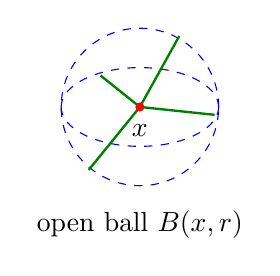
\begin{tikzpicture}
\draw[blue, dashed] (3,0) circle [radius=1cm];
\draw[blue, dashed] (2,0) arc (180:360:1 and 0.5);
\draw[blue, dashed] (4,0) arc (0:180:1 and 0.5);
\node[] () at (3,-0.3) {\(x\)};
\draw[green!50!black, line width=0.3mm] (3,0) -- (3.5,0.9);
\draw[green!50!black, line width=0.3mm] (3,0) -- (2.5,0.4);
\draw[green!50!black, line width=0.3mm] (3,0) -- (2.35,-0.8);
\draw[green!50!black, line width=0.3mm] (3,0) -- (3.95,-0.1);
\draw[red, fill] (3,0) circle [radius=0.5mm];
\node[] () at (3,-1.5) {open ball \(B(x,r)\)};
\end{tikzpicture}
\end{center}
Note that every radius of the open ball \(B(x,r)\) (\gc{green} line segments in
the picture above) is homeomorphic to the interval \([0,r)\subseteq \R\), which
is connected by \Cref{lma:int-conn}. Since connectedness is a topological
property, every radius is connected. Furthermore, the intersection of all the
radii is \(\{x\}\), thus nonempty. Noting the open ball \(B(x,r)\) is indeed
the union of all the radii (with nonempty intersection), we conclude by
\Cref{prp:conn-union-nonemp-int-conn} that the open ball \(B(x,r)\) is
connected.

Since \(T\) contains \(x\), it must be the union of all connected sets
containing \(x\) by \Cref{prp:conn-comp-union}.  Hence, we must have
\(B(x,r)\subseteq T\). Thus, \(T\) is open in \(\R^n\).
\end{enumerate}
\end{pf}
\end{enumerate}
